For evaluation purposes, we have used HDF5's \textit{h5perf} performance tool~\cite{h5perf}. It allows configuring various parameters, such as the number of processes to run the test with, number of datasets to be created in the file, amount of data contributed by each process per dataset, amount of data read/written by a process in a single I/O call (transfer size) etc. For our measurements, we created 10 datasets in the file, and the total file size was 64 GB or more.

All tests were performed on the Lustre parallel file system~\cite{lustre} on the Atlas cluster at University of Dresden. The file system has 12 OSTs with a stripe size of 1MB. The file system is connected to the compute nodes using an SDR Infiniband link. It should be noted that the file system is in production and subject to demanding and varying workload. We present here the average bandwidth values of 3 runs, though in certain cases, we have seen significant variation.
The cluster has 92 AMD Opteron nodes with 64 cores each and 64 to 512 GB memory. 

We have performed tests with 1,2,4,8,32 and 64 processes. We spawned a maximum of 4 processes per node.
Reads and writes are either contiguous or interleaved; processes either access contiguous locations in file or execute a strided pattern.
We compare the performance of the default MPI-IO driver, our plugin, and the PLFS MPI-IO driver (ad\_plfs). 

In Figure~\ref{write_contig}, we show the write performance for a transfer size of 1MB for contiguous writes, for varying number of processes. It can be seen that the plugin regularly outperforms MPI-IO. However, as we increase the number of processes, its performance falls below that of ad\_plfs. Figure~\ref{read_contig} shows the performance of contigous reads for an unaligned transfer size. The plugin again outperforms MPI-IO, but the performance of ad\_plfs is the best for 64 processes. 
%Figure~\ref{write_interleaved} shows the performance of unaligned writes for a maximum of 8 processes. We set the transfer size here to be 10 bytes more than 1MB. Also, the writes here are interleaved as opposed to contiguous. We see a similar pattern, where the plugin outperforms MPI-IO, but is not as good as that of ad\_plfs for 8 processes. 
Figure~\ref{write_collective} compares the performance of MPI-IO with that of the plugin for collective, unaligned, interleaved writes for a maximum of 8 processes. It is important to note that the plugin outperforms MPI-IO in collective mode. We have not been able to obtain results for collective ad\_plfs due to resource restrictions.   

Overall, our results show that although the plugin generally shows good performance, it does not scale as well as we increase the number of processes. This is due to the fact that since we are directly making calls to the PLFS API, the metadata overhead seems to be high. We have all processes participating in file open and close operations, which for large problem sizes can add siginificant overhead. Hence, for future work, we plan to use ad\_plfs directly in the plugin which can overcome this performance drawback, since ad\_plfs has collective optimizations in open and close. It should however be noted that MPI libraries like Volpex-MPI~\cite{volpex}, which do not have MPI-IO as part of their MPI library, could make use of a plugin that does not rely on MPI-IO.  

\begin{figure}[!t]
\centering
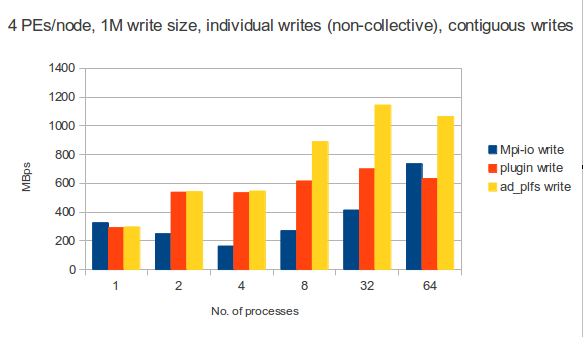
\includegraphics[width=2.5in]{4PEs_node_1M_contig_ind_writes}
\caption{Performance of contiguous writes}
\label{write_contig}
\end{figure}

\begin{figure}[!t]
\centering
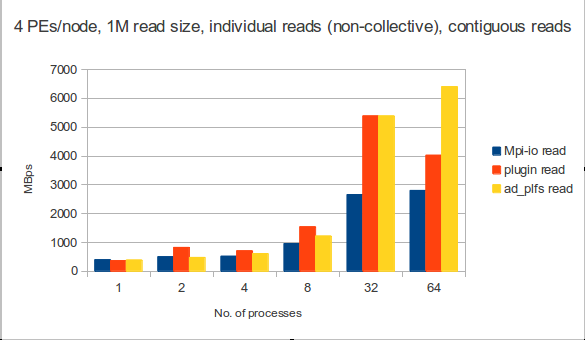
\includegraphics[width=2.5in]{4pes_node_1m_ind_read}
\caption{Performance of contiguous reads}
\label{read_contig}
\end{figure}

%\begin{figure}[!t]
%\centering
%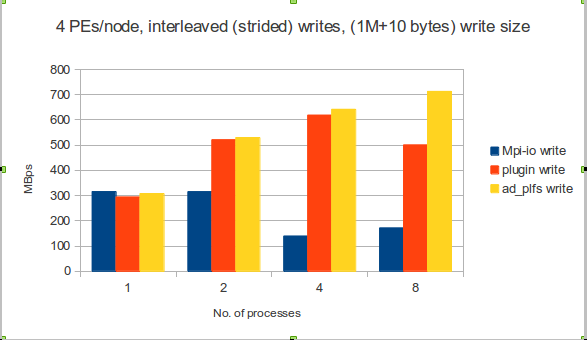
\includegraphics[width=2.5in]{interleaved_1M10_4pes_writes_noncoll}
%\caption{Performance of interleaved writes}
%\label{write_interleaved}
%\end{figure}

\begin{figure}[!t]
\centering
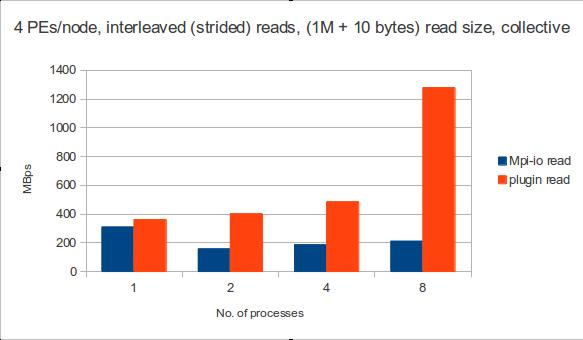
\includegraphics[width=2.5in]{4pes_interleaved_1m10_coll_reads}
\caption{Performance of collective writes}
\label{write_collective}
\end{figure}


